%---------------------------------------------------------------------
%
%                  Project Name: Radar System Network Report
%
%---------------------------------------------------------------------
%
%                 created by LuoMin <luomin5417@gmail.com>
%
%                        Last-modified: 2018-5-18
%
%---------------------------------------------------------------------

\documentclass[a4paper,12pt]{report}
\usepackage{etex}
\usepackage{ctex}
%\usepackage{xeCJK}
\usepackage{times}
\usepackage{setspace}
\usepackage{fancyhdr}
\usepackage{graphicx}
\usepackage{wrapfig}
\usepackage{array}  
\usepackage{fontspec,xunicode,xltxtra}
\usepackage{titlesec}
\usepackage{titletoc}
\usepackage[titletoc]{appendix}
\usepackage[top=30mm,bottom=30mm,left=20mm,right=20mm]{geometry}
\usepackage{cite}
\usepackage{listings}
\usepackage{caption,subcaption}
\usepackage[framed,numbered,autolinebreaks,useliterate]{mcode} % 插入代码
\usepackage{xeboiboites}
\usepackage{amsmath,amssymb}
\usepackage{hyperref}

\RequirePackage{tkz-network}

\hypersetup{hidelinks}

\XeTeXlinebreaklocale "zh"
\XeTeXlinebreakskip = 0pt plus 1pt minus 0.1pt

%---------------------------------------------------------------------
%	页眉页脚设置
%---------------------------------------------------------------------
\fancypagestyle{plain}{
	\pagestyle{fancy}      %改变章节首页页眉
}

\pagestyle{fancy}
\lhead{\kaishu~宜通华盛~}
\rhead{\kaishu~研发部~}
\cfoot{\thepage}

%---------------------------------------------------------------------
%	章节标题设置
%---------------------------------------------------------------------
\titleformat{\chapter}{\centering\zihao{-1}\heiti}{第\chinese{chapter}章}{1em}{}
\titlespacing{\chapter}{0pt}{*0}{*6}

%---------------------------------------------------------------------
%	摘要标题设置
%---------------------------------------------------------------------
\renewcommand{\abstractname}{\zihao{-3} 摘\quad 要}

%---------------------------------------------------------------------
%	参考文献设置
%---------------------------------------------------------------------
\renewcommand{\bibname}{\zihao{2}{\hspace{\fill}参\hspace{0.5em}考\hspace{0.5em}文\hspace{0.5em}献\hspace{\fill}}}

%---------------------------------------------------------------------
%	引用文献设置为上标
%---------------------------------------------------------------------
\makeatletter
\def\@cite#1#2{\textsuperscript{[{#1\if@tempswa , #2\fi}]}}
\makeatother

%---------------------------------------------------------------------
%	目录页设置
%---------------------------------------------------------------------
\titlecontents{chapter}[0em]{\songti\zihao{-4}}{\thecontentslabel\ }{}
{\hspace{.5em}\titlerule*[4pt]{$\cdot$}\contentspage}
\titlecontents{section}[2em]{\vspace{0.1\baselineskip}\songti\zihao{-4}}{\thecontentslabel\ }{}
{\hspace{.5em}\titlerule*[4pt]{$\cdot$}\contentspage}
\titlecontents{subsection}[4em]{\vspace{0.1\baselineskip}\songti\zihao{-4}}{\thecontentslabel\ }{}
{\hspace{.5em}\titlerule*[4pt]{$\cdot$}\contentspage}

%---------------------------------------------------------------------
%	公式设置
%---------------------------------------------------------------------
%%define the newthem environment
\newboxedtheorem[small box style={fill=blue!20,draw=black, 
    rounded corners},
    big box style={fill=blue!10,draw=orange,thick,rounded corners},
    headfont=\bfseries]%
    {proposition}{公式}{somecounter} 

%---------------------------------------------------------------------
%   生成大纲
%---------------------------------------------------------------------

\begin{document}
%---------------------------------------------------------------------
%	封面设置
%---------------------------------------------------------------------
\begin{titlepage}
	\begin{center}
		
    
\includegraphics[width=0.9\textwidth]{figure//etws.png}\\
    \vspace{40mm}
    \textbf{\zihao{2}\kaishu{ETWS-1609雷达系统}}\\[0.8cm]
    \textbf{\zihao{2}\kaishu{网络管理设计方案}}\\[3cm]
    
	\vspace{\fill}
	
\setlength{\extrarowheight}{3mm}
{\songti\zihao{3}	
\begin{tabular}{rl}
	
	{\makebox[4\ccwd][s]{部\qquad 门:}}& ~\kaishu 研发部\\
	
	{\makebox[4\ccwd][s]{编\qquad 制:}}& ~\kaishu 罗敏 \\ 

\end{tabular}
 }\\[2cm]
\vspace{\fill}
\zihao{4}
使用\LaTeX 撰写于\today
	\end{center}	
\end{titlepage}

%---------------------------------------------------------------------
%  摘要页
%---------------------------------------------------------------------
\begin{abstract}
\begin{spacing}{1.5}
	{\zihao{-4}
	本文主要是关于雷达系统远程控制网络的体系结构设计,目的是实现全国各地雷达系统的远程监
	测与控制,主要是从两个方面来考虑如何设计实现,第一是从可操作性方面来考虑,因整个控制
	网连接的设备较多,特别是雷达设备甚至可能是位于郊区等人迹罕至的地方,将所有的接入设备
	都连接固定IP专网接口是不太现实的,而且费用过高,方案必须符合实际具有可操作性。第二个
	是从安全性的角度,整个系统分布与全国各地,且连接的雷达用户各不相同,需要考虑用户之间
	的隔离,以及防止非法的网络入侵破坏雷达系统工作。要实现这两个目的,通过可以采用VPN技
	术,将分布于各地的雷达设备、控制主机和后端管理服务器配置成为一个虚拟专网,这样的设计
	只需要位于后端的VPN服务器一个固定IP,其它设备只需要连接普通的互联网服务便可以实现目
	的,费用低廉具有可操作性,且VPN的数据传输采用了多重加密技术可以有效防止数据泄露。

	\textbf{关键字}:\quad 远程监控 \quad VPN \quad 虚拟专网 \quad 安全性
	}
\end{spacing}
\end{abstract}

%---------------------------------------------------------------------
%  目录页
%---------------------------------------------------------------------
\tableofcontents % 生成目录

%---------------------------------------------------------------------
%  第一章
%---------------------------------------------------------------------
\chapter{设计方案}
\setcounter{page}{1}
\begin{spacing}{1.5}
\songti\zihao{-4}

\section{系统结构}
要对整个雷达系统进行网络设计,则需要先弄楚整个雷达系统的结构组成,下面主要对雷达系统的特
点进行了一些总结:
\begin{itemize}
\itemsep=3pt
\parskip=0pt
\setlength{\itemindent}{1em} 
\item 系统庞大设备多,包括雷达、控制服务器、监控摄像头、UPS设备等等
\item 设备分散位于全国各地,后期可能还会不停的在各个地方扩展
\item 需要时时监控设备工作情况,随时获取雷达数据
\end{itemize}

整个系统的结构如图1.1所示:
\begin{figure}[hbtp]
	\centering
	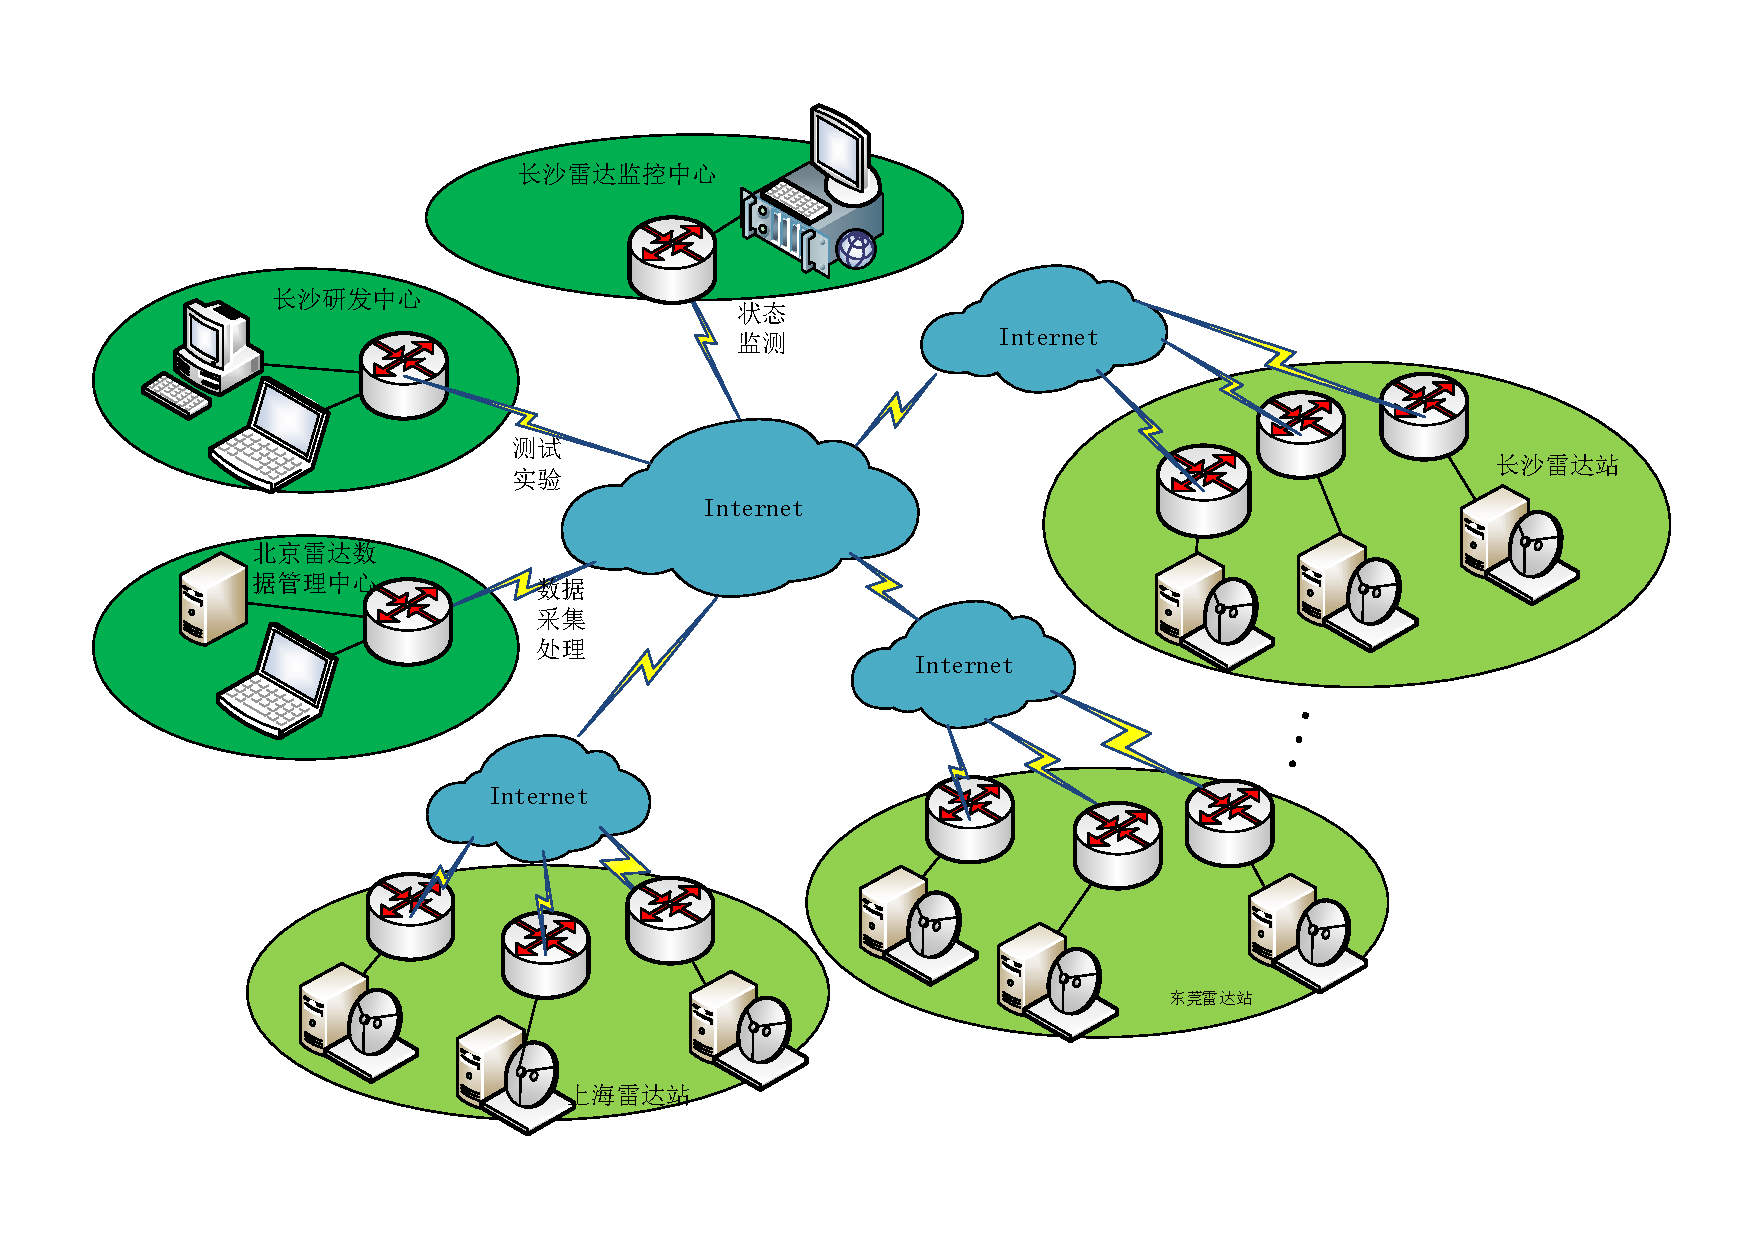
\includegraphics [width=1.0\textwidth]{figure//RadarSystem.pdf}
	\caption{雷达系统结构图}\label{RadarSystem}
\end{figure}

在图1.1可以看到雷达系统组成结构复杂,每个站点有多台雷达,不同站点的雷达也是各自分散的,
根据目前的发展情况,后续还会增加更多的雷达站点,除了雷达站点之外雷达系统的监控管理中心
在长沙,长沙的研发中心也会有访问雷达站点进行实验测试的需求,北京雷达数据管理中心则是主要
需要从各个雷达站点读取数据进行雷达数据的处理。

\section{网络设计}
上一节简单的介绍了整个雷达系统的结构,本节根据雷达系统的结构,进行网络管理方案设计。针对
目前的情况和现有的技术,本文决定采用VPN技术组建私有专网,具体组网方案如图1.2所示:
\begin{figure}[hbtp]
	\centering
	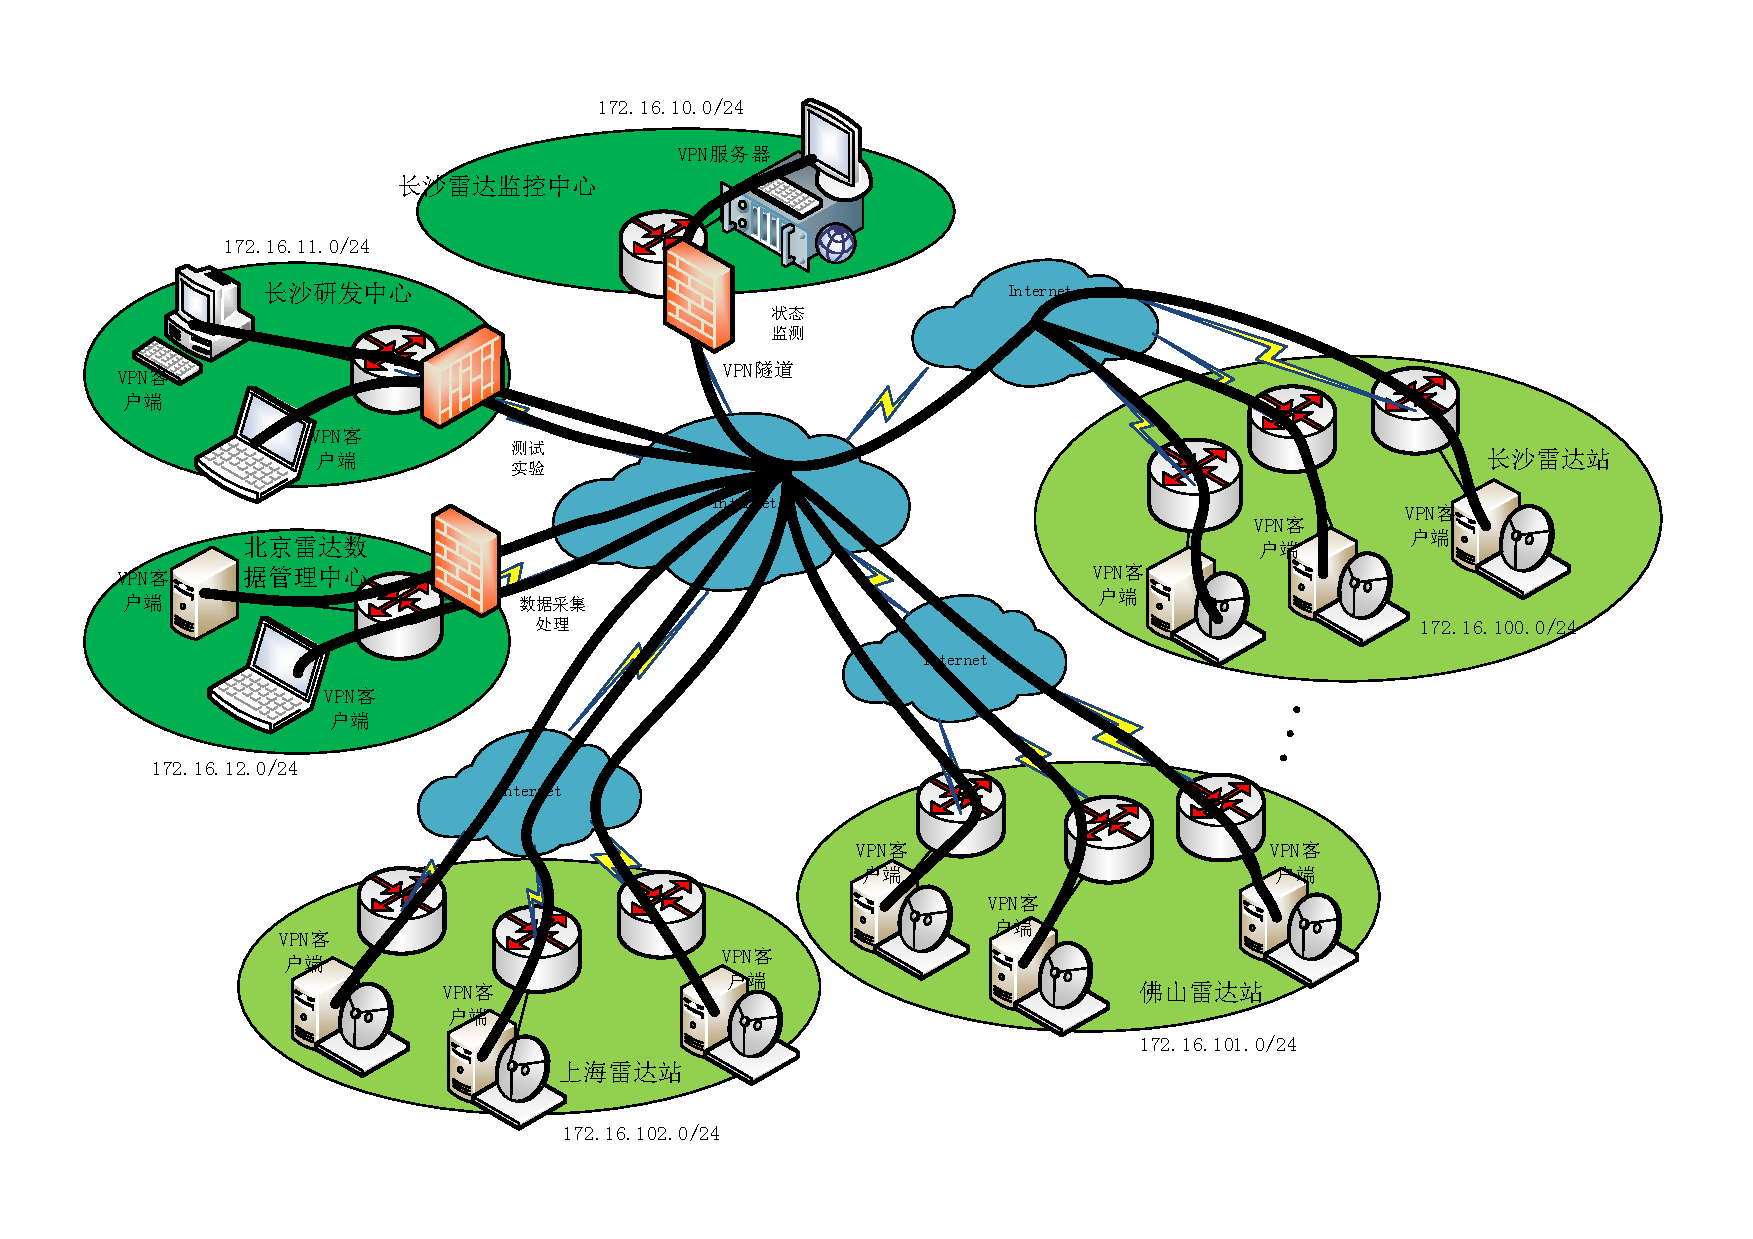
\includegraphics [width=1.0\textwidth]{figure//RadarNet.pdf}
	\caption{雷达系统网络设计}\label{RadarNet}
\end{figure}

在长沙雷达管理中心设置一台VPN服务器,来提供VPN服务管理,其它的网络节点,则通过VPN客户端
远程加入VPN网络,因此长沙雷达管理中心需要一个专网IP,以便其它节点可以方便访问。为了系统
安全还需要进行网络隔离,各个雷达站之间不能相互访问,同时需要在各个管理中心添加防火墙,防
止雷达站访问到网络中心。

目前考虑没有能够满足要求的集成VPN路由器,只能采用在雷达设备的内部服务器上配置VPN客户端,
后期可以考虑我司自主设计一个多功能网关设备作为雷达站点的控制网关,届时可以将VPN客户端
配置在多功能集成网关上。

\section{网络划分}
在图1.2中标注的网络地址是指

\end{spacing}


%---------------------------------------------------------------------
%  第二章
%---------------------------------------------------------------------
\chapter{网络安全}

%---------------------------------------------------------------------
%  第三章
%---------------------------------------------------------------------
\chapter{工具软件}

%---------------------------------------------------------------------
%  第四章
%---------------------------------------------------------------------
\chapter{配置步骤}

\begin{spacing}{1.5}
\section{实验目的}
本实验的目的是验证olsr协议报文时钟与网络中报文数据量之间的关系。
\section{实验工具}
同上一实验。
\section{实验设计}
实验拓扑仍然采用图1.1所示,通过设置不同的hello和tc报文时钟,然后计算整个拓扑中OLSR协议的报文流通量再除以整个测试时间计算式如下:

\begin{proposition}[OLSR协议流量计算]
	数学表达式:
	\[(\sum_{i=1}^n X_i)/t \overset{\textnormal{p.s.}}{\longrightarrow} \mathbb{E} (X_i) .\]
	其中X$i$表示i节点发出的报文总数,t表示拓扑测试时间。
\end{proposition}

根据公式,分别设置了四组hello和tc报文时钟,分别是(2.0, 5.0),(1.0, 2.5), (0.5, 1), (0.2, 0.4),然后运行过程中使用wireshark统计
了各个节点的数据流量,记录了拓扑测试时间。


\section{数据分析}
在图2.1中记录了四组时钟情况下的流通量,根据图可以看到,随着hello报文和tc报文时钟的变短,报文量快速上升,基本上呈现一个线性上升的关
系,而且上升趋势比较平缓,处于可以接受的范围内。
\begin{figure}[hbtp]
\centering
\begin{tikzpicture}
	\draw [ycomb, color = blue!20, line width = 0.5 cm]
	plot coordinates{(1.5,0.557) (3,1.101) (4.5,2.735) (6,5.217)};
	\coordinate [label=above:{$5.57$}](A) at (1.5,0.6);
	\coordinate [label=above:{$11.01$}](A) at (3,1.2);
	\coordinate [label=above:{$27.35$}](A) at (4.5,3);
	\coordinate [label=above:{$52.19$}](A) at (6,5.5);
	\draw (1.5, -0.1) node [below] {2.0/5.0} -- (1.5, 0.1)
	(3, -0.1) node [below] {1.0/2.5} -- (3, 0.1)
	(4.5, -0.1) node [below] {0.4/1.0} -- (4.5, 0.1)
	(6, -0.1) node [below] {0.2/0.4} -- (6, 0.1);
	%\foreach \i in {1,2,3,4}
	%\draw (-0.1, \i) node [left] {\i} -- (0.1, \i);
	\draw (-0.1, 1) node [left] {10} -- (0.1, 1)
	(-0.1, 2) node [left] {20} -- (0.1, 2)
	(-0.1, 3) node [left] {30} -- (0.1, 3)
	(-0.1, 4) node [left] {40} -- (0.1, 4)
	(-0.1, 5) node [left] {50} -- (0.1, 5)
	(-0.1, 6) node [left] {60} -- (0.1, 6);

	\draw [<->] (0,6.5) node [above] {$kbps$}
	-- (0,0)
	-- (6.5,0) node [right] {$hello/tc$} ;
\end{tikzpicture}
\caption{报文数据流量}
\end{figure}


同时我们关心单位时间内报文流量的情况在当hello和tc报文分别设置到(0.2, 0.4),根据图1.2的(d)子图可以看到,路由切换基本能够满足在
300ms左右完成切换,且此时流量维持在52kbps左右,这样的流量大小和切换时延是能够接受的。

\section{实验结论}
本实验结论:一定程度上缩短hello报文和tc报文的时钟,可以加速路由表的切换,且拓扑中所增加的报文流量是能够接受和可以预期的。
\end{spacing}

%---------------------------------------------------------------------
%  实验感想
%---------------------------------------------------------------------
\titleformat{\chapter}{\centering\zihao{-1}\heiti}{第\chinese{chapter}章}{1em}{}
\chapter{实验总结}
\begin{spacing}{1.5}
通过本次仿真实验加深了对于OLSR协议的理解,也从理论上指导了在设备上调试运行OLSR协议,并且为后续针对OLSR协议的改进打下了良好的基
础。
\end{spacing}

%---------------------------------------------------------------------
%  参考文献设置
%---------------------------------------------------------------------
\addcontentsline{toc}{chapter}{参考文献}

\begin{thebibliography}{99}
\songti \zihao{-4} 	
	\bibitem{NS3.web}
	https://www.nsnam.org/
	\bibitem{rfc3626.olsr}
	Network Working Group. OLSR: Optimized Link State Routing Protocol, 2003.
	
\end{thebibliography}

%---------------------------------------------------------------------
%  附录设置
%---------------------------------------------------------------------
\titleformat{\chapter}{\heiti\Large}{附录~\Alph{chapter}}{11pt}{\Large}
\titlespacing{\chapter}{0pt}{*-4}{*4}

\lstset{breaklines}                %自动将长的代码行换行排版
\lstset{extendedchars=false}
\lstset{language=Matlab}
\renewcommand{\thechapter}{附录\Alph{chapter}.} 
\appendix
\begin{appendix}
	
	
\chapter{数据表}
\zihao{-4}\songti
\begin{spacing}{1.5}
\begin{enumerate}
\item 路由表记录文件
\item 各节点抓包文件
\end{enumerate}
\end{spacing}


\chapter{程序代码}
\zihao{-4}\songti
\begin{spacing}{1.5}
下面是ns3仿真的C++程序,分别设置了各个节点的属性和测试过程,具体可以参考代码内容。
\begin{lstlisting}[language=c++]
/* -*-  Mode: C++; c-file-style: "gnu"; indent-tabs-mode:nil; -*- */
/*
	* Copyright (c) 2009 University of Washington
	*
	* This program is free software; you can redistribute it and/or modify
	* it under the terms of the GNU General Public License version 2 as
	* published by the Free Software Foundation;
	*
	* This program is distributed in the hope that it will be useful,
	* but WITHOUT ANY WARRANTY; without even the implied warranty of
	* MERCHANTABILITY or FITNESS FOR A PARTICULAR PURPOSE.  See the
	* GNU General Public License for more details.
	*
	* You should have received a copy of the GNU General Public License
	* along with this program; if not, write to the Free Software
	* Foundation, Inc., 59 Temple Place, Suite 330, Boston, MA  02111-1307  USA
	*
	*/

//
// This program configures a grid (default 5x5) of nodes on an
// 802.11b physical layer, with
// 802.11b NICs in adhoc mode, and by default, sends one packet of 1000
// (application) bytes to node 1.
//
// The default layout is like this, on a 2-D grid.
//
// n20  n21  n22  n23  n24
// n15  n16  n17  n18  n19
// n10  n11  n12  n13  n14
// n5   n6   n7   n8   n9
// n0   n1   n2   n3   n4
//
// the layout is affected by the parameters given to GridPositionAllocator;
// by default, GridWidth is 5 and numNodes is 25..
//
// There are a number of command-line options available to control
// the default behavior.  The list of available command-line options
// can be listed with the following command:
// ./waf --run "wifi-simple-adhoc-grid --help"
//
// Note that all ns-3 attributes (not just the ones exposed in the below
// script) can be changed at command line; see the ns-3 documentation.
//
// For instance, for this configuration, the physical layer will
// stop successfully receiving packets when distance increases beyond
// the default of 500m.
// To see this effect, try running:
//
// ./waf --run "wifi-simple-adhoc --distance=500"
// ./waf --run "wifi-simple-adhoc --distance=1000"
// ./waf --run "wifi-simple-adhoc --distance=1500"
//
// The source node and sink node can be changed like this:
//
// ./waf --run "wifi-simple-adhoc --sourceNode=20 --sinkNode=10"
//
// This script can also be helpful to put the Wifi layer into verbose
// logging mode; this command will turn on all wifi logging:
//
// ./waf --run "wifi-simple-adhoc-grid --verbose=1"
//
// By default, trace file writing is off-- to enable it, try:
// ./waf --run "wifi-simple-adhoc-grid --tracing=1"
//
// When you are done tracing, you will notice many pcap trace files
// in your directory.  If you have tcpdump installed, you can try this:
//
// tcpdump -r wifi-simple-adhoc-grid-0-0.pcap -nn -tt
//

#include "ns3/core-module.h"
#include "ns3/mobility-module.h"
#include "ns3/wifi-module.h"
#include "ns3/internet-module.h"
#include "ns3/olsr-helper.h"

#include "ns3/netanim-module.h"

using namespace ns3;

NS_LOG_COMPONENT_DEFINE ("WifiSimpleAdhocGrid");

void ReceivePacket (Ptr<Socket> socket)
{
	while (socket->Recv ())
	{
		NS_LOG_UNCOND ("Received one packet!");
	}
}

static void GenerateTraffic (Ptr<Socket> socket, uint32_t pktSize,
								uint32_t pktCount, Time pktInterval )
{
	if (pktCount > 0)
	{
		socket->Send (Create<Packet> (pktSize));
		Simulator::Schedule (pktInterval, &GenerateTraffic,
							socket, pktSize,pktCount - 1, pktInterval);
	}
	else
	{
		socket->Close ();
	}
}


int main (int argc, char *argv[])
{
	std::string phyMode ("DsssRate1Mbps");
	double distance = 500;  // m
	uint32_t packetSize = 1000; // bytes
	uint32_t numPackets = 100;
	uint32_t numNodes = 4;  // by default, 5x5
	uint32_t sinkNode = 0;
	uint32_t sourceNode = 3;
	double interval = 1.0; // seconds
	bool verbose = false;
	bool tracing = false;
	double HelloInterval = 2.0;
	double TcInterval = 5.0;
	double MidInterval = 5.0;
	double HnaInterval = 5.0;

	CommandLine cmd;

	cmd.AddValue ("phyMode", "Wifi Phy mode", phyMode);
	cmd.AddValue ("distance", "distance (m)", distance);
	cmd.AddValue ("packetSize", "size of application packet sent", packetSize);
	cmd.AddValue ("numPackets", "number of packets generated", numPackets);
	cmd.AddValue ("interval", "interval (seconds) between packets", interval);
	cmd.AddValue ("verbose", "turn on all WifiNetDevice log components", verbose);
	cmd.AddValue ("tracing", "turn on ascii and pcap tracing", tracing);
	cmd.AddValue ("numNodes", "number of nodes", numNodes);
	cmd.AddValue ("sinkNode", "Receiver node number", sinkNode);
	cmd.AddValue ("sourceNode", "Sender node number", sourceNode);
	cmd.AddValue ("hellointerval", "OLSR Routing Protocol hello packet interval", HelloInterval);
	cmd.AddValue ("tcinterval", "OLSR Routing Protocol Tc packet interval", TcInterval);
	cmd.AddValue ("midinterval", "OLSR Routing Protocol Mid interval", MidInterval);
	cmd.AddValue ("hnainterval", "OLSR Routing Protocol Hna interval", HnaInterval);

	cmd.Parse (argc, argv);
	// Convert to time object
	Time interPacketInterval = Seconds (interval);

	// disable fragmentation for frames below 2200 bytes
	Config::SetDefault ("ns3::WifiRemoteStationManager::FragmentationThreshold", StringValue ("2200"));
	// turn off RTS/CTS for frames below 2200 bytes
	Config::SetDefault ("ns3::WifiRemoteStationManager::RtsCtsThreshold", StringValue ("2200"));
	// Fix non-unicast data rate to be the same as that of unicast
	Config::SetDefault ("ns3::WifiRemoteStationManager::NonUnicastMode",
						StringValue (phyMode));

	NodeContainer c;
	c.Create (numNodes);

	// The below set of helpers will help us to put together the wifi NICs we want
	WifiHelper wifi;
	if (verbose)
	{
		wifi.EnableLogComponents ();  // Turn on all Wifi logging
	}

	YansWifiPhyHelper wifiPhy =  YansWifiPhyHelper::Default ();
	// set it to zero; otherwise, gain will be added
	wifiPhy.Set ("RxGain", DoubleValue (-10) );
	// ns-3 supports RadioTap and Prism tracing extensions for 802.11b
	wifiPhy.SetPcapDataLinkType (WifiPhyHelper::DLT_IEEE802_11_RADIO);

	YansWifiChannelHelper wifiChannel;
	wifiChannel.SetPropagationDelay ("ns3::ConstantSpeedPropagationDelayModel");
	wifiChannel.AddPropagationLoss ("ns3::FriisPropagationLossModel");
	wifiPhy.SetChannel (wifiChannel.Create ());

	// Add an upper mac and disable rate control
	WifiMacHelper wifiMac;
	wifi.SetStandard (WIFI_PHY_STANDARD_80211b);
	wifi.SetRemoteStationManager ("ns3::ConstantRateWifiManager",
								"DataMode",StringValue (phyMode),
								"ControlMode",StringValue (phyMode));
	// Set it to adhoc mode
	wifiMac.SetType ("ns3::AdhocWifiMac");
	NetDeviceContainer devices = wifi.Install (wifiPhy, wifiMac, c);

	MobilityHelper mobility;
	mobility.SetPositionAllocator ("ns3::GridPositionAllocator",
									"MinX", DoubleValue (0.0),
									"MinY", DoubleValue (0.0),
									"DeltaX", DoubleValue (distance),
									"DeltaY", DoubleValue (distance),
									"GridWidth", UintegerValue (4),
									"LayoutType", StringValue ("RowFirst"));
	//mobility.SetMobilityModel ("ns3::ConstantPositionMobilityModel");
	mobility.SetMobilityModel ("ns3::ConstantVelocityMobilityModel");
	mobility.Install (c);

	c.Get (0)->GetObject<MobilityModel> ()->SetPosition (Vector (0, 500, 0));
	c.Get (0)->GetObject<ConstantVelocityMobilityModel> ()->SetVelocity (Vector (20, 0, 0));

	// Enable OLSR
	OlsrHelper olsr;
	Ipv4StaticRoutingHelper staticRouting;

	Time t_HelloInterval = Seconds (HelloInterval);
	olsr.Set("HelloInterval", TimeValue(t_HelloInterval));

	Time t_TcInterval = Seconds (TcInterval);
	olsr.Set("TcInterval", TimeValue(t_TcInterval));

	Time t_MidInterval = Seconds (MidInterval);
	olsr.Set("MidInterval", TimeValue(t_MidInterval));

	Time t_HnaInterval = Seconds (HnaInterval);
	olsr.Set("HnaInterval", TimeValue(t_HnaInterval));


	Ipv4ListRoutingHelper list;
	list.Add (staticRouting, 0);
	list.Add (olsr, 10);

	InternetStackHelper internet;
	internet.SetRoutingHelper (list); // has effect on the next Install ()
	internet.Install (c);

	Ipv4AddressHelper ipv4;
	NS_LOG_INFO ("Assign IP Addresses.");
	ipv4.SetBase ("10.1.1.0", "255.255.255.0");
	Ipv4InterfaceContainer i = ipv4.Assign (devices);

	TypeId tid = TypeId::LookupByName ("ns3::UdpSocketFactory");
	Ptr<Socket> recvSink = Socket::CreateSocket (c.Get (sinkNode), tid);
	InetSocketAddress local = InetSocketAddress (Ipv4Address::GetAny (), 80);
	recvSink->Bind (local);
	recvSink->SetRecvCallback (MakeCallback (&ReceivePacket));

	Ptr<Socket> source = Socket::CreateSocket (c.Get (sourceNode), tid);
	InetSocketAddress remote = InetSocketAddress (i.GetAddress (sinkNode, 0), 80);
	source->Connect (remote);

	if (tracing == true)
	{
		AsciiTraceHelper ascii;
		wifiPhy.EnableAsciiAll (ascii.CreateFileStream ("wifi-simple-adhoc-grid.tr"));
		wifiPhy.EnablePcap ("wifi-simple-adhoc-grid", devices);
		// Trace routing tables
		Ptr<OutputStreamWrapper> routingStream = Create<OutputStreamWrapper> ("wifi-simple-adhoc-grid.routes", std::ios::out);
		olsr.PrintRoutingTableAllEvery (Seconds (0.1), routingStream);
		Ptr<OutputStreamWrapper> neighborStream = Create<OutputStreamWrapper> ("wifi-simple-adhoc-grid.neighbors", std::ios::out);
		olsr.PrintNeighborCacheAllEvery (Seconds (0.1), neighborStream);

		// To do-- enable an IP-level trace that shows forwarding events only
	}

	// Give OLSR time to converge-- 30 seconds perhaps
	Simulator::Schedule (Seconds (120.0), &GenerateTraffic,
						source, packetSize, numPackets, interPacketInterval);

	// Output what we are doing
	NS_LOG_UNCOND ("Testing from node " << sourceNode << " to " << sinkNode << " with grid distance " << distance);

	Simulator::Stop (Seconds (123.0));

	AnimationInterface anim("olsr-adhoc.xml");

	Simulator::Run ();
	Simulator::Destroy ();

	return 0;
}
\end{lstlisting}
\end{spacing}
\end{appendix}
		

\end{document}